\chapter{Introdução a IHC}\label{cap:cap1}

\begin{flushright}
	\textit{
		Persistência é a irmã gêmea da excelência. \\
		Uma é a mãe da qualidade, a outra é a mãe do tempo.
	} \\
	
	\textbf{Marabel Morgan}
\end{flushright}

Ao parar por um instante e numerar a quantidade de ferramentas computacionais que são utilizadas no dia a dia, aparentemente parece uma tarefa simples. Talvez, em um dia apenas, esse número não seja tão alarmante. Mas, ao listar todas que podem ser utilizadas durante um mês, ou até um ano, como: telefone celular, computadores, controle remoto, maquinas de refrigerante, caixas eletrônicos, impressores, videogames..., a lista se torna interminável. Ao analisar portanto este exemplos, percebe-se que as tecnologias de informação e comunicação (TICs) estão ocupando espaço importante nas nossas vidas. Segundo \citeonline{barbosa2010IHC} as TICs, são sistemas computacionais compostos por hardware, software e meios de comunicação desenvolvidos para interagirem com pessoas. Estas tecnologias permitem criar sistemas computacionais embutidos nos mais diferentes dispositivos eletrônicos, que combinam poder computacional e meios de comunicação. Para os autores, a evolução e a disseminação dessas tecnologias alcançaram um nível em que é difícil encontrar pessoas que ainda não tiveram direta ou indiretamente contato com elas, independente de classe social, do nível de escolaridade e do local onde moram.

Assim, neste novo mundo tecnológico, o interesse na forma com que ocorre a interação entre o ser humano e o computador tem se expandido proporcionalmente a medida em que se amplia a quantidade de usuários que utilizam computadores para realizar as mais diversas tarefas. Justamente neste ponto que se encontra a área de estudo da Interação Humano-Computador (IHC), que tem seu foco na qualidade de uso e no impacto que estas interações causam na vida do ser humano \cite{barbosa2010IHC}. Baseando-se nestes acontecimentos, pode-se dizer que a interação do usuário com o computador tornou-se tão importante quanto o processamento realizado por ele e, apoiando-se neste pressuposto, pesquisadores buscam desenvolver técnicas e ferramentas para facilitar o \textit{design} de interfaces de acordo com as necessidades do usuário, utilizando para isso os conceitos que englobam a área de IHC \cite{barbosa2010IHC}.

\section{Interação, interface e \textit{design}} \label{section:interacao-e-interface-e-design}
Para que se possa entender alguns termos muito utilizados nos textos a seguir, em especial, três destes devem ser compreendido com maior destque, os quais são: interação, interface e \textit{design}.

Desde os primórdios da humanidade a interação é fator central na relação do ser humano com o meio em que vive e com seus semelhantes. O contato com a natureza e os relacionamentos são necessidades essenciais ao homem que busca conhecer e satisfazer seus anseios. 

Em determinado momento da história chegou-se a conclusão que a Interação é um termo mais amplo em conceitos do que a Interface. Imagine um grande conjunto chamado interação que, para existir, necessita de um elemento que permita a comunicação – a interface.  

Já nos meios digitais, a interação do homem com o computador segue princípios semelhantes tendo como meio de comunicação, entre estes dois elementos, as interfaces. Em síntese, interface pode ser definida como o meio que permite a interação entre usuário e sistema, ou seja, a interatividade acontece por meio da interface gráfica, que funciona como o meio de contato que permite a interação \cite{lemos2015cibercultura}. 

Assim, em determinado momento da história, chegou-se a conclusão que a Interação é um termo mais amplo em conceitos do que a Interface. Imagine um grande conjunto chamado interação que, para existir, necessita de um elemento que permita a comunicação – a interface. O resultado disso é que, entendendo a interação, será mais fácil projetar a interface \cite{IrlaRebelo}.

\begin{figure}[H]
    \centering
    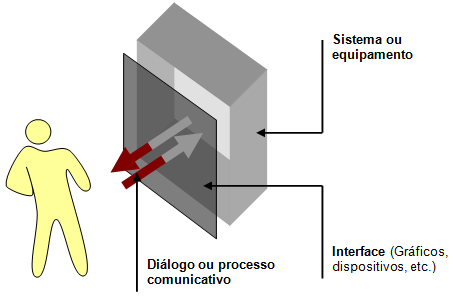
\includegraphics[scale=0.6]{imagens/interfaceinteracao.jpg}
    \caption{Representação simplificada do processo de interação e sua relação com a interface}
    \legend{Fonte: \cite{IrlaRebelo}}
    \label{fig:interface-interacao}
\end{figure}

Logo, com a inserção do computador no cotidiano das pessoas, pesquisas em \textit{design} foram desenvolvidas para aprimorar as interfaces buscando melhorar a interação ao longo do tempo. Portanto, a relação entre interação, interface e \textit{design}, está no fato que, uma melhor interação entre o sujeito e a interface é proporcionada por um melhor \textit{design} \cite{lemos2015cibercultura}.

\section{Evolução das interfaces} \label{section:evolucao-das-interfaces}
No início do desenvolvimento de sistemas computacionais a interface de comunicação entre o ser humano e o computador era feita por meio de sistemas mecânicos como chaves e cartões perfurados. Um exemplo desta tecnologia do passado pode ser recordada com o uso que o exército dos Estados Unidos fez do ENIAC \textit{(Electronic Numerical Integrator Analyzer and Computer)}, apresentado na Figura \ref{fig:eniac}, na qual a forma de interação era feita por meio de aproximadamente 6.000 (seis mil) chaves manuais e, ao invés de teclas, toda a inserção de dados era realizada por meio de cartões de cartolina perfurados, que armazenavam poucas operações cada um. Uma equipe preparava os cartões, incluindo as operações a serem realizadas, formando uma pilha, outra trocava os cartões no leitor do ENIAC, e uma terceira ``traduzia'' os resultados também impressos em cartões \cite{Morimoto2011}. Logo, os engenheiros desenvolviam os sistemas computacionais para que eles próprios pudessem utilizar sendo a interface mais funcional do que amigável.

\begin{figure}[H]
    \centering
    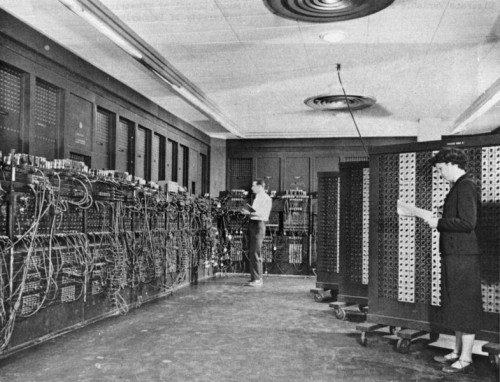
\includegraphics[scale=0.6]{imagens/eniac.jpg}
    \caption{ENIAC (foto do acervo do exército dos Estados Unidos).}
    \legend{Fonte: \cite{Morimoto2011}}
    \label{fig:eniac}
\end{figure}

Contudo, com o surgimento dos computadores pessoais no final dos anos 70 (setenta) e início dos anos 80 (oitenta), o \textit{design} de interação passa a existir juntamente com um novo conceito de interface, gerando assim novos desafios, sendo um dos maiores, o desenvolvimento de interfaces que pudessem ser utilizadas por qualquer pessoa e não somente especialistas \cite{rogers2005design}. 

Já em meados dos anos 90, surgem novas tendências de desenvolvimento tecnológico como: redes, computadores, sensores, computação móvel, entre outros. Estas tecnologias que emergiram tornaram o desenvolvimento de aplicações para diversas pessoas uma realidade. Muitas empresas perceberam que suas equipes multidisciplinares de \textit{design} deveriam ser expandidas incluindo assim outros profissionais como: \textit{designer} industrial, de filmes, dentro tantos outros. Todos estes novos papéis possuem um único objetivo em comum, projetar a nova geração de sistemas interativos \cite{rogers2013design}. 

A partir dos anos 2000, as possibilidades alcançadas pela capacidade emergente dos hardwares demostram que os desafios da interação estão indo além do puro contato do homem com o computador. Neste sentido, engenheiros devem estar aptos a configurar, montar e programar até eletrodomésticos para que eles possam se comunicar uns com os outros \cite{rogers2013design}, ou seja, o estágio atual, também conhecido como ``Internet das Coisas'', está fundamentado pela conectividade e interatividade entre pessoas, informações, processos e objetos, por meio de tecnologias que possibilitam acesso à rede por qualquer pessoa, de qualquer lugar, a qualquer tempo, utilizando quaisquer dispositivos, incluindo equipamentos multifuncionais como sensores inteligentes, tais como eletrodomésticos, automóveis, roupas, a partir de aplicações que se adaptam dinamicamente às necessidades dos usuários. \cite{lacerda2015necessidade}. 

Portanto, os desafios para a criação de interfaces que facilitem a comunicação humano-computador torna-se um desafio constante e crescente. E, em meio a isso, IHC tornou-se a área de estudo que tem como foco os aspectos relacionados à interação entre usuários e computadores, como também, entre o usuários e estes diversos meios que surgem, buscando entender as diversas visões do usuário perante os sistemas, com o objetivo de facilitar o seu dia a dia. 

\section{Atores e visões sobre os sistemas}
Existem diversos atores envolvidos no desenvolvimento e uso dos sistemas computacionais. Para \citeonline{falbo2011engenharia}, dá-se nome de ator a um papel desempenhado por entidades físicas (pessoas, organizações ou outros sistemas) que interagem com o sistema em questão da mesma maneira, procurando atingir os mesmos objetivos. Contudo, quando se fala em atores em IHC, deve-ser ter um pouco de cuidado, pois, atores neste contexto, são apenas pessoas, que utilizam os sistemas computacionais para alcançar seus objetivos. Neste sentido, fabricantes de hardware, de software, vendedores, profissionais de suporte e manutenção, provedores de acesso à Internet, produtores de conteúdo, usuários, organizações, dentre outros, são possíveis partes interessadas, as quais costumam ser denominadas \textit{stakeholders}. Cada um enxerga a tecnologia sob um ponto de vista diferente, enfatizando alguns aspectos em detrimento de outros \cite{barbosa2010IHC}. Portanto, para \citeonline{barbosa2010IHC}, a identificação dos diferentes atores o stakeholders envolvidos e a articulação dos seus interesses e pontos de vista são importantes desafios no desenvolvimento de tecnologia, ou no caso de IHC, melhorar a interação por meios de um melhor \textit{design} de interfaces.

\section{Abordagem de desenvolvimento}
Grande parte da Computação e, em particular, a subárea de Engenharia de Software, está interessada na construção de sistemas interativos mais eficientes, robustos, livres de erros, e de fácil manutenção. Por outro lado, a área de Interação Humano-Computador (IHC) está interessada na qualidade de uso desses sistemas e no seu impacto na vida dos seus usuários. Apesar de fortemente relacionados, a construção e o uso de um artefato ocorrem em contextos distintos e seguem lógicas diferentes, envolvendo pessoas diversas. Por ter a qualidade de construção como prioritária, grande parte da Computação costuma conceber um sistema interativo de ``dentro para fora'', como pode ser visto na Figura \ref{fig:abordagens-de-desenvolvimento}a, isto é, conceber primeiro representações de dados, algoritmos que processam esses dados, arquitetura do sistema e tudo mais que permite um sistema interativo funcionar \cite{barbosa2010IHC}.

Para conceber um sistema interativo mais adequado ao mundo onde será inserido,
a área de IHC (e, sob alguns aspectos, também a área de Engenharia de Requisitos)
busca seguir uma abordagem de ``fora para dentro'', como visto na Figura \ref{fig:abordagens-de-desenvolvimento}b. Nessa abordagem, o projeto de um sistema interativo começa investigando os atores envolvidos, seus interesses, objetivos, atividades, responsabilidades, motivações, os artefatos utilizados, o domínio, o contexto de uso, dentre outros, para depois identificar oportunidades de intervenção na situação atual, a forma que a intervenção tomará na interface com o usuário e, finalmente, como o sistema viabiliza essa forma de intervenção \cite{barbosa2010IHC}.

\begin{figure}[H]
    \centering
    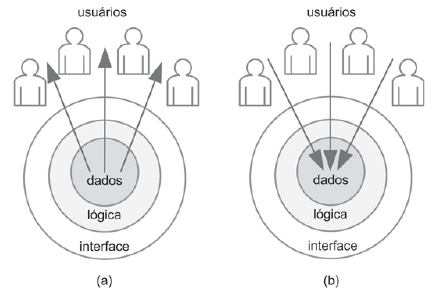
\includegraphics[scale=0.5]{imagens/abordagem-desenvolvimento.png}
    \caption{Abordagem de desenvolvimento (a) de ``dentro para fora'' e (b) de ``fora para dentro''.}
    \legend{Fonte: \cite{barbosa2010IHC}}
    \label{fig:abordagens-de-desenvolvimento}
\end{figure}

\section{Objetos de estudo}
E fato, e demostrado ate este momento, que o objetivo de IHC é melhorar os sistemas computacionais objetivando uma melhor interação dos seres humanos com as interfaces. Assim, melhorar a experiência de uso e a qualidade da interação exige investigar o uso de sistema interativo os quais envolvem diversos objetos os quais são: 


\begin{itemize}
    \item \textbf{natureza da interação humano-computador:} investiga quando o sistema será usado e o que ocorre durante o uso de um sistema interativo pelo usuário.
    \item \textbf{uso de sistemas interativos situado em contexto:} investiga onde o sistema será usado: a cultura, sociedade, linguagem, ambiente físico e o contexto de uso.
    \item \textbf{características humanas:} investiga o usuário, a capacidade cognitiva do usuário para processar informações e aprender a utilizar o sistema, e as suas características físicas como visão, audição, movimentação para aproveitar suas capacidades e respeitar seus limites.
    \item \textbf{arquitetura de sistemas computacionais e interfaces com usuários:} investiga o sistema, tecnologias e dispositivos que possibilitem facilitar e melhorar a interação entre sistemas e usuários.
    \item \textbf{processo de desenvolvimento:} investiga métodos, técnicas e ferramentas para avaliação e construção de interfaces.
\end{itemize}

\section{Áreas relacionadas à IHC}

IHC é uma área do conhecimento que utilizada outras áreas fora da Computação
para conhecer de forma mais ampla os fenômenos que envolvem o uso de sistemas computacionais. Estas áreas são definidas pela multidisciplinaridade que envolve especialista e profissionais de diversas áreas como:

\begin{itemize}
    \item psicologia;   
    \item sociologia;
    \item antropologia;
    \item sistemas de informação;
    \item ciências da computação;
    \item design gráfico;
    \item ergonomia.
\end{itemize}

Alguns conhecimentos e técnicas importados de outras áreas além da Computação
são adaptados às necessidades de IHC. Por exemplo, a Psicologia utiliza extensamente
entrevistas para ter acesso às concepções, emoções e subjetividade das
pessoas. Isso é muito mais profundo e complexo que a utilização mais frequente de
entrevistas em IHC, através das quais normalmente investigamos a compreensão sobre
um domínio, opiniões sobre certos sistemas interativos e o que ocorreu durante
uma experiência de uso para avaliação da interface com usuário. Algumas técnicas
de apresentação de conteúdo estático, como as utilizadas em jornais, revistas e livros, foram adaptadas em IHC para lidar com a dinâmica da interface, bem como conteúdos hipermídia \cite{barbosa2010IHC}.

\section{Benefícios de IHC}

Inicialmente, foi apresentado as TICS, as quais, fazem parte, diretamente ou indiretamente de quase todos os afazeres diários. Neste sentido, segundo \citeonline{barbosa2010IHC} deve-se então buscar o melhor aproveitamente das características humanas e o poder computacional para desenvolvermos sistemas interativos que melhorem a vida das pessoas, trazendo bem-estar, aumentando sua produtividade, satisfazendo suas necessidades e desejos, e respeitando suas limitações e valores. Melhorando a qualidade de uso, pode-se então contribuir para:


\begin{itemize}
    \item Aumentar a produtividade das pessoas;
    \item Reduzir o número de erros cometidos durante o uso e a gravidade deles;
    \item Reduzir o custo de treinamento, pois as pessoas poderão aprender durante o uso;
    \item Reduzir o custo de suporte técnico, pois as pessoas terão menos problemas para usar o sistema;
    \item Aumentar as vendas e a fidelidade do cliente à sua marca! (Vide Apple);
    \item Reduzir o custo de desenvolvimento;
    \item Tornar o mundo um lugar melhor de viver!
\end{itemize}

\section{Conclusão}
Interagir diariamente com produtos diferentes que possuem impactos diferentes na vida do ser humano faz parte do cotidiano de todos. O contato com esses produtos não depende somente da forma com que foram projetados, mas também do ambiente da cultura onde este está inserido, como também, das atividades que são executadas no momento em que é utilizado. 

Um ponto importante que deve ser levado em consideração ao projetar uma interface esta no fato de que, se a interação ocorrer de maneira negativa para o usuário, ele poderá sentir-se com raiva, estressado ou até mesmo procurar outros produtos que substitua aquele inicial. O grande fator responsável para que isso aconteça consiste no fato que os produtos são construídos, geralmente, deixando de lado o fator humano.

IHC coloca o usuário em primeiro lugar desde o início do projeto até a sua finalização, passando por vários momentos de avaliação, os quais serão apresentados em posteriores capítulos. Assim, é preciso conhecer quem são os usuários, quais são as suas culturas, hábitos, desejos, capacidades e limitações. Ao levar esses fatores em consideração, a qualidade e a experiência de uso são melhoradas. 

\section{Exercício de fixação}

\begin{enumerate}
	\item Defina interação, interface e \textit{design} segundo os conceitos apresentados em aula, como também, explique a relação entre os três conceitos.
	\item Em aula foi discutimos sobre quem são os atores para IHC. Explique o que são atores segundo os conceitos de IHC e argumento sobre o porquê devemos entender os atores durante o desenvolvimento das interfaces.
	\item Duas abordagem de desenvolvimento foram apresentadas, a ``de dentro para fora'' e a ``de fora para dentro''. Ilustre com suas palavras, o porquê, para IHC, ``de fora para dentro'' é a abordagem indicada.
	\item IHC é uma área do conhecimento que utiliza outras área para ampliar a visão do pesquisador sobre os fenômenos no uso de sistemas computacionais. Explique essa razão utilizando para este fim os benefícios de IHC.
	\item \textbf{(Desafio)} Busque em sua cidade problemas que podem ser solucionados pelo uso de algum tipo de aplicativo. Descrava o problema e explique o motivo que o(a) levou a soluciona-lo por meio de um software. 
\end{enumerate}


